\chapter{Problem Definition and Analysis}\label{sec:problem-definition-analysis}
In this section first the problem definition will be introduced. Next, the analysis of this problem will be discussed. Last, the requirements following from this analysis and the wishes of the client are presented.

\section{Problem Definition}
As discussed in the previous sections the hypthesis the client proposed is if a semantic association of cities can give insight into on the actual relationships and strengths between cities. This hypothesis introduces the problem how software could be used to find and analyse these semantic associations. This lead to the following problem definition:\\

\begin{quote} 
\centering 
\textit{How can open data be leveraged such that a metric for the strength of relationships between cities can be defined and visualised?}
\end{quote}

\section{Problem Analysis}
The problem can be divided into four sub-problems that need to be addressed to solve the problem. These are Filtering, Classification, Storing Data and  Data Visualisation \& Export. 

\subsubsection{Filtering}
The first sub-problem is filtering, which means searching through the available text data to find co-occurrences of cities and discarding text data that does not contain co-occurrences. This should reduce the amount of data and thereby potentially speed up the rest of process.

\subsubsection{Classification}
The sub-problem that arises after filtering is how to determine what relationships can be extracted from the text-data, this will be referred to as the classification of the text-data. This requires a method that reliably and efficiently processes the text-data and can be tuned to the clients wishes, meaning that the classification should output what the client desires. 

\subsubsection{Storing Data}
Next, when the classification sub-problem is addressed the need arises to store the data and determine the strength of the relationships. 

\subsubsection{Data Visualisation \& Export}
When these three sub-problems have been successfully solved the last sub-problem that is left is how to combine the stored data and present it to a user, this means visualising and/or exporting the data in an accessible way.

\section{Requirement Analysis}\label{sec:reqs-analysis}
In this section, we first present user stories that were created together with the client. Next, we define the design goals. Then, we list the requirements which followed from the user stories and which the application should meet. To do so, we use the MoSCoW method\cite{clegg1994case} as a prioritisation technique. Lastly, we discuss the design decisions that follow from the design goals and the requirements.

\subsection{User Stories}
Together with the client, several user stories are identified for interaction with the system. These are listed below.

As a user:
\begin{enumerate}
    \item I want to be able to see all the identified relations between all cities, so that I can reason about interesting patterns.
    \item I want to be able to access extracted relations in an Excel file. I want this to be available per relation type and as a total of all relations, so that I can apply my own models on the data.
    \item I want to be able to see relation strengths, which can be expressed by counting the relations.
    \item I want to be able to (de)select cities in the user interface, so that I can create a network of cities connected with relations. A network of cities consists of the cities as nodes and the different types of relationships as edges between them.
    \item I want to be able to (de)select relations between cities in the user interface, so that I can inspect only the relations I am interested in. For example, as a user I might only be interested in the Transportation relationship between Amsterdam and Rotterdam.
    \item I want to be able to change the colours associated with the different relation types, so that I can adjust the styling to my own preferences.
    \item I want to be able to export an image of the map that I composed in the user interface so that I can use it for presentations, papers or educational purposes
\end{enumerate}

\subsection{Design Goals} \label{sec:design-goals}
The high-level design goals for this project have been provided by the client. These serve as a guideline to determine the priority label of the specific requirements as defined in section \ref{sec:reqs}. The design goals are listed below, ordered by priority.

\subsubsection{credible} The results of the project will be used in research on intercity relations. Therefore, the results must be reliable and verifiable. This means that the application should produce the same results given the same input and it should be possible to manually access the input to verify the output of the application.
\subsubsection{understandable} The results of the application should be visually understandable, in order to make it easy for the client to deduce conclusions. 
\subsubsection{scalable} During the project a TU Delft server will be used with a limited amount of resources. Therefore only .nl pages will be used as input to limit the amount of data storage and processing power needed. However, allowing for investigating other domains would greatly help the client in a later stadium, which means that the system would have to be scalable where possible. For example, using a dedicated database which can be spread across clusters.
\subsubsection{plugable} It might be interesting for the user to let the application perform analysis on different data sets without the need of a developer. So if possible within the time constraints the application should be able to use any form of textual input data.
\subsubsection{exportable} Besides making the results available visually, all the relevant numeric data should also be exportable, for example in CSV format, so the client is able to process the data beyond the system.
\subsubsection{fast development} Because of the time constraints of the project we need a fast development cycle. As a result of that, choices regarding tools, applications and programming languages are to be made with the time constraint taken into account.


\subsection{Product Requirements}\label{sec:reqs}
As mentioned in the introduction of section \ref{sec:reqs-analysis} we will be using the MoSCoW method prioritisation technique. Four levels of priority are defined: must have, should have, could have and would have (also known as would like). We also differentiate between functional and non-functional requirements. 

\subsubsection{Must Have}
Requirements labelled as must have are key to the minimal performance of the application. If they are not met, the application can be considered a failure.

\begin{enumerate}
    \item Data that is of relevance for the UrbanSearch project, should be mined from the Common Crawl web corpus (see section\ref{sec:commoncrawl}) and stored for further processing/access.
    \item There has to be a way to export the relations between cities.
    \item A machine learning algorithm should analyse and label the collected data to extract different types of relations that are important for intercity relations.
    \item A front-end should be built for the project. This front-end should visualise basic relations and statistics and can be used for presentations and educational purposes.
    \item Several statistically important aspects of intercity relations should be extracted from the data set. These statistics should be easily accessible and visualised to the end user. Furthermore, it should be easy to extend or update the list of statistics that are associated with a relation.
\end{enumerate}
\iffalse
\begin{enumerate}
    \item A user must be able to select place names.
    \item The system must display a map with the before mentioned places and the important connection they have to other places.
    \item A user must be able to choose a connection between two places and get information about what kind of relations they have.
    \item The strength of all relations must be displayed.
    \item The user must be able to export the found connections and their strengths between places.
    \item Data, that is of relevance for the UrbanSearch project, should be mined from the Common Crawl web corpus and stored for further processing/access. 
    \item A machine learning algorithm should analyse the collected data and attempt to identify different types of relations that are important for intercity relations.
    \item Several statistically important aspects of intercity relations should be extracted from the data set. These statistics should be easily accessible and understandable to the end user. Which statistics are important is one of the research topics of this project, so it should be easy to extend/update the list of statistics that are associated with a relation.

\end{enumerate}
\fi
\subsubsection {Should Have}
"Should have" requirements are those that greatly improve system performance and/or usability but might not fit in the available development time.

\begin{enumerate}
    \item Relations between cities should be accessible hierarchically. This means that there is the possibility to explore a relation and, provided that this relation has sub-types associated with it, the relation can be expanded in the different sub-types of the relation.
    \item It should be possible to retrain the machine-learning algorithm on demand by feeding it a set of labelled documents.
    \item It should be possible to add large data sets, e.g. with more than 1 million documents, on which the system can perform its data mining routines. This way a data set can be created that contains potentially interesting information for intercity relations.
    \item The application should be able to deal with the fact that the same city can have different names in different languages/dialects. It should still be able to extract and group relevant data correctly (e.g. 'The Hague' and 'Den Haag' should be viewed as the same city).
\end{enumerate}
\iffalse
\begin{enumerate}
    \item The user should be able to (de)select cities.
    \item The application should be able to use multiple data sets.
    \item The application should be able to group the relations (e.g. 'fish-trade' and 'finance' to economy, 'medicine' to health-care etc).
    \item The user should be able to 'zoom' on places in order to see more/less connections to other places.
    \item The user should be able to interact with the map so only relations of a certain type will be shown.
    \item The user should be able to select whether relative or absolute strengths should be shown.
    \item A user should be able to export an image of the map.
    \item Relations between cities should be accessible hierarchically. This means that there is the possibility to query a relation and, provided that this relation has sub-types associated with it, the relation can be expanded in the different sub-types of the relation.
    \item A machine learning algorithm should be able to group different relationships that are strongly connected to each other.
    \item It should be possible to add big data sets on which the system can perform its data mining routines. This way a data set can be created that contains potentially interesting information for intercity relations.
    \item The software should understand that the same city can have different names in different languages/dialects. It should still be able to extract and group relevant data correctly (e.g. 'The Hague' and 'Den Haag' should be viewed as the same city).
\end{enumerate}
\fi
\subsubsection {Could Have}
Requirements labelled as "could have" are useful and should be included in the system if time and resources permit.

\begin{enumerate}
    \item The system should use Delpher (see also section \ref{sec:delpher}), a collection of over 60 million digitalised newspaper articles, books and magazines in the Netherlands, of age ranging from the seventeenth century to now, to characterise relationships between a region and cities outside that region. For example, the local newspaper of the province Gelderland writing about the city of Alkmaar. These relationships are either simple or complex information flows. A newspaper mentioning a city is considered a simple information flow, whereas multiple cities mentioned in a single document is a complex information flow. Both simple and complex flows reside on the basic properties of the document, such as the publication date. An illustration of this is given in figure \ref{fig:infoflow}.
    \item The relations that are extracted from the data by the machine learning algorithm have to be visualised in a way that makes it easy to compare the different relations for the end user. For example, a split-screen comparison in the user interface or an export of graphs comparing selected relations.
\end{enumerate}
\begin{figure}
    \centering
    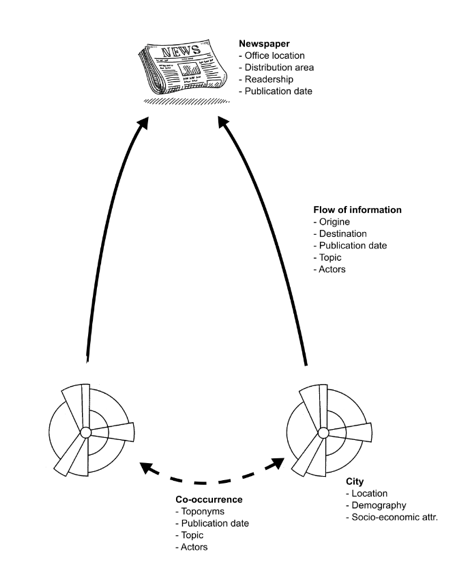
\includegraphics{informationflow}
    \caption{Solid lines represent simple information flows, whereas the dashed line is a complex connection of information. We focus on the part depicted by the dashed line.}
    \label{fig:infoflow}
\end{figure}
\iffalse
\begin{enumerate}
    \item The application could be able to use international names.
    \item A front-end should be build for the UrbanSearch system. This front-end should visualise basic relations and statistics and can be used for presentations or educational purposes
    \item The software should use Delpher to characterise relationships between a region and cities outside that region based on newspapers in those regions, aggregated over the past 50 years. These relationships are either simple or complex information flows. Simple information flows consist of a newspaper located in city i publishing about city j, whereas complex information flows are co-occurrences of cities in an article.
    \item The relations that are extracted from the data by the machine learning algorithm and the relations provided by the CBS have to be visualised in a way that makes it easy to compare the different relations for the end user.
\end{enumerate}
\fi
\subsubsection {Would Like}
"Would like" requirements have been agreed upon to be not important to include within the current time schedule. However, they can be included in future releases.

\begin{enumerate}
    \item The application would be able to show all connections of all places on the map at the same time.
    \item Using data from top-level domains other than \texttt{.nl}.
\end{enumerate}

\subsection{Design Decisions}
To be able to have a fast development cycle and leverage our experience we chose to develop the application using Python. 
We plan to not only test the code we deliver thoroughly, but also to cross-validate the obtained results. The specifics of this validation protocol will be discussed in section \ref{sec:validation_protocol}.